\documentclass[cclicense]{hmcthesis}

\usepackage{util}
\usepackage{math}

\usepackage{makeidx}
\makeindex

\newcommand*{\X}{\mathfrak{X}}
\newcommand*{\F}{\mathcal{X}}
\newcommand*{\Mod}{\mathcal{M}}
\newcommand*{\Bin}{\mathcal{B}}
\newcommand*{\vbar}{\;\big\vert\;}
\newcommand*{\mle}{\theta_{\text{mle}}}
\DeclareMathOperator{\Mixt}{Mixt}
\DeclareMathOperator{\intr}{int}
\DeclareMathOperator{\Sec}{Sec}
\DeclareMathOperator*{\argmax}{arg\ max}

\newcommand*{\parop}[1]{\frac{\partial}{\partial #1}}

\numberwithin{equation}{section}

\title{Thesis Draft}
\author{Aaron Pribadi}
\thesisyear{2012}

\advisor{Michael Orrison}
\reader{Weiqing Gu}

\begin{document}

\frontmatter

\maketitle

\tableofcontents


\chapter{Abstract}
    This will be an abstract.

\chapter{Acknowledgements}
    There will be acknowledgements.

\mainmatter

\chapter{Introduction}

\section{Binary Values and Statistical Models}

\section{Algebraic Statistics}

    Algebraic statistics is a relatively new field that examines statistical
    questions using algebraic geometry and commutative algebra.  Once a problem
    has been cast in the language of algebra, a number of computational tools
    can be brought to bear.  For example, one of the early papers in the field
    analyzed contingency tables using Monte Carlo sampling computed with Gröbner
    bases \citep{DS98}.

    Algebraic statistics also offers a geometric point of view on statistical
    models; the tendency is toward intrinsically defined objects in lieu of
    explicit coordinate systems.  In this light, algebraic statistics might be
    seen as in the tradition of information geometry, a field pioneered in the
    1980s that applied the techniques of Riemannian geometry to probability
    models (see for example \citep{Ama}).

    An introduction to the field of algebraic statistics may be found in the
    collection of lecture notes \citep{DSS08}.  Algebraic statistics has also
    been applied to computational biology \citep{ASCB}.

    Our goal is to examine a particular statistical model, the Restricted
    Boltzmann Machine, from the point of view of algebraic statistics building
    from prior work in that direction, especially \citep{CMS09}.  The Restricted
    Boltzmann Machine has recently become the centerpiece of certain
    developments in the machine learning community \citep{Hin07}, and basic
    questions about its geometry remain unanswered.  
    
    We begin in Section 2 by explaining the geometric framework of our approach.
    In Section 3 we present the Restricted Boltzmann Machine and some known
    results, and in Section 4 we develop our own characterization of the model
    in the hope that it will prove illuminating.

\chapter{The Geometry of Statistical Models}
    \section{The Probability Simplex}

    We consider probability distributions over finite sets.  The space of all
    such distributions corresponds to a geometric object.
    
    \begin{definition} 
        \index{simplex}
        The \emph{probability simplex} of dimension $N$ (also
        called the \emph{standard simplex}) is the space
        \[
            \Delta_N = 
            \left\{(x_1, \ldots, x_{N+1}) \vbar \sum_{i=1}^{N+1} x_i= 1, x_i \ge 0 \right\} 
            \subset
            \R^{N+1}.
        \]
        If the appropriate dimension is either clear in context or irrelevant we
        may simply write $\Delta$, omitting the subscript.
    \end{definition}
    A \emph{simplex} in general is the image of a standard simplex under any
    affine transformation.  Low-dimensional simplices are familiar objects;
    $\Delta_0$ is a point, $\Delta_1$ is a line segment, $\Delta_2$ is a
    triangle, and $\Delta_3$ is a tetrahedron.
    \begin{figure}[H]
        \centering
        \scalebox{1}{ 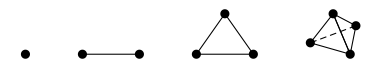
\includegraphics[scale=0.5]{images/simplices.png} }
        \caption{Low-dimensional simplices.}
    \end{figure}
    \noindent A random variable $X$ with $N+1$ possible values corresponds to a point $x =
    (x_1, \ldots, x_{N+1})$ contained in the simplex $\Delta_N$ in a natural
    way; if $X$ takes values in $\{1, \ldots, N+1\}$, we set $P(X = i) = x_i$.
    We usually identify a probability distribution with its corresponding
    point in the probability simplex.  
    
    Statisticians are often concerned with families of probability
    distributions.  We identify such families with geometric spaces.
    \begin{definition}
    By the phrase \emph{statistical model}, we mean a subset $\Mod \subset
    \Delta$ of a probability simplex.
    \end{definition}
    \noindent A statistical model may be parametrized by a map $f: U \to
    \Delta$, for some space $U$ of parameters.  Usually, the space of parameters
    is a subset of a real affine space $\R^d$, and parametrizations are
    differentiable almost everywhere.  In the context of algebraic statistics,
    the parametrization is usually a rational function.
    \begin{example}
    A random variable $X$ following a binomial distribution with size $N$ and
    parameter $\lambda \in [0,1]$ takes a value $k \in \{0,\ldots, N\}$ with
    probability
    \[
        P_\lambda[X = k] = {N \choose k} \lambda^k(1-\lambda)^{n-k}.
    \]
    This is the number of heads produced by $n$ `coin tosses', where $\lambda$
    is the probability of a head.  The map $\lambda \mapsto P_\lambda$
    determines a parametrized statistical model $\{P_\lambda : \lambda \in [0,1]
    \} \subset \Delta_N$. The statistical model is a curve, i.e. a
    one-dimensional subspace, of the simplex.  

    Take $N=2$, which simulates two coin flips.  The three coordinates of a
    point in the model measure the probabilities that zero, one, and two heads
    will occur, respectively.
    \begin{figure}[H]\label{fig:binomial}
        \centering
        \vspace*{-0.2cm}
        \scalebox{1}{ 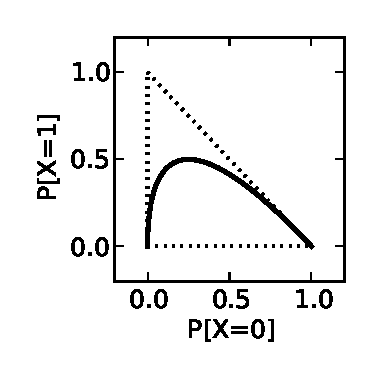
\includegraphics[scale=0.7]{images/binomial.pdf} }
        \vspace*{-0.5cm}
        \caption{The binomial statistical model for $N=2$.}
    \end{figure}
    \noindent As the parameter $\lambda$ varies over $[0,1]$, the statistical
    model traces out the curve 
    \[
        \lambda \longmapsto \big((1-\lambda)^2, 2\lambda(1-\lambda), \lambda^2\big)
    \]
    in the simplex $\Delta_2$.  The final coordinate
    $P[X=2]$ does not need to be displayed, because we can compute it from the
    first two coordinates.  
    \end{example}
    
\section{Maximum Likelihood Estimation}

    Suppose that some data are taken from an unknown distribution, and that we
    want to model the data using some statistical model $\Mod \subset \Delta$.
    A distribution matches the data well if the data are relatively probable
    given the distribution.  Throughout this section we use discrete
    distributions, though our definitions can be made more general.

    Let $\Mod = \{P_\theta : \theta \in U\}$ be a parametrized statistical
    model. A random variable $X$ distributed according to some $P_\theta$ has
    the probability mass function $p_\theta(x) = P_\theta[X = x]$.  Suppose that
    we have data $Z = \{z_1, \ldots, z_n\}$.  The data are generally assumed to
    be independent and identically distributed according to some unknown true
    distribution in $\Mod$.
    
    \begin{definition}
    The \emph{likelihood function} of $\theta \in U$ given the data $Z$ is
    \[
        L(\theta; Z) = \prod_{i=1}^n p_\theta(z_i).
    \]
    It is the probability that the observed data $Z$ would occur if the
    observations were independent and identically distributed and following
    $P_\theta$.  The \emph{log-likelihood function} is
    \[
        l(\theta; Z) = \sum_{i=1}^n \log p_\theta(z_i)
    \]
    and is often used in place of the likelihood function because it is additive.
    \end{definition}
    \begin{definition}
    The \emph{maximum likelihood estimate} of the true parameter is the
    parameter 
    \[
        \mle = \argmax_{\theta \in U} L(\theta; Z)
    \]
    that maximizes the likelihood (or equivalently the log-likelihood) of the
    data.
    \end{definition}

    The maximum likelihood estimate is not always well-defined.  The estimate
    might not be unique, as the maximal likelihood could be attained multiple
    times.  The estimate  might not even exist, as the model could be a
    non-closed subset of the simplex.  In practice, it is possible that an
    optimal parameter is not necessary and that a merely good one is sufficient.
    Standard numerical optimization techniques, e.g. those based on gradient
    descent or Newton's method, can handle many models.  A more precise
    knowledge of the geometry of a statistical model, however, can make maximum
    likelihood estimation easier.

\section{Solutions to the Likelihood Equations}

    Here, we give a flavor of how algebro-geometric techniques can be applied to
    maximum likelihood estimation.  Our exposition follows Section 3.3 of
    \citep{ASCB} and Section 2.1 of \citep{DSS08}.

    Suppose that $g: U \to \Delta_{N-1}$ is a rational parametrization of a
    statistical model, where $U$ is an open subset of $\R^d$.  By rational, we
    mean that each component of $g(\theta) = (g_1(\theta), \ldots, g_N(\theta))$
    is a rational function with rational coefficients in its argument $\theta
    \in U \subset \R^d$.  Maximum likelihood estimation then amounts to
    maximizing the function
    \[
        l(\theta) = \sum_{i=1}^N u_i \log g_i(\theta)
    \] 
    where $u_i$ is the number of times event $i$ has occurred in the observed
    data.

    Every local and global maximum $\theta \in U$ is a solution to the
    likelihood equations
    \begin{equation}\label{eq:lik}
        \frac{\partial l}{\partial\theta_j}
        =
        \sum_{i=1}^N 
        \frac{u_i}{g_i} 
        \cdot
        \frac{\partial g_i}{\partial \theta_j}
        = 0
        \qquad
        \text{for $j = 1,\ldots,d$}.
    \end{equation}
    The likelihood equations in \eqref{eq:lik} are again rational functions of
    $\theta$.  Solving the equations involves `clearing denominators' and
    solving the polynomial equations
    \begin{equation}\label{eq:lik-clear}
        \sum_{i=1}^N 
        u_i \cdot g_1 \cdots \widehat{g_i} \cdots g_N
        \frac{\partial g_i}{\partial \theta_j}
        = 0
        \qquad
        \text{for $j = 1, \ldots, d$}
    \end{equation}
    where $\widehat{g_i}$ indicates that the $i$-th factor is omitted.  The
    equations \eqref{eq:lik-clear}, however, introduce extraneous solutions, for
    example when $g_a(\theta) = g_b(\theta) = 0$ for any $a \ne b$.

    Algebraic geometry offers a principled way to solve the likelihood
    equations.  (For a brief introduction to affine and projective varieties, see
    Section \ref{sec:varieties} of the appendix.)  Consider the ideal $I \subset \R[\theta_1,
    \ldots, \theta_d]$ generated by the polynomial expressions in \eqref{eq:lik-clear}
    \[
        I = \adel[\Bigg]{
            \sum_{i=1}^N u_i \cdot g_1 \cdots \widehat{g_i} \cdots g_N
            \frac{\partial g_i}{\partial \theta_j}
        }_{j=1}^d
        .
    \]
    Let $h$ be the product of all polynomials appearing in the denominators of
    the rational equations in \eqref{eq:lik}.  The \emph{saturation ideal} of
    $I$ with respect to $h$ is defined
    \[
        (I : h^\infty) = \cdel[\big]{
            f \in \R[\theta_1, \ldots, \theta_d]
            \;\big\vert\;
            fh^k \in I
            \quad
            \text{for some non-negative integer $k$}
        }.
    \]
    We can then consider the variety corresponding to the saturation ideal.  The
    points in $V(I : h^\infty) \cap U$ are all solutions to the likelihood
    equations.  In the case that there are only finitely many solutions, passing
    to the saturation ideal removes all extraneous solutions.

    The referenced works \citep{ASCB} and \citep{DSS08} include examples of
    computing the variety $V(I : h^\infty)$ with the software package
    \texttt{Singular}.  An overview of the techniques used to solve such
    polynomial equations, e.g. Gröbner bases, resultants, and elimination, is
    given in the text \citep{CLO05} on computational algebraic geometry.
% 
% \section{Implicit Models}

    % In the context of algebraic statistics, we usually look at statistical
    % models that are semialgebraic sets.

    % If a statistical model is a semi algebraic set, then we can pass to its
    % Zariski closure in affine space, or we can embed it in projective space
    % and takes its Zariski closure there.

    % A simplex is the locus of a finite collection of polynomial equations
    % and polynomial inequalities and therefore is a semialgebraic set.

    % Then we can solve the likelihood equations, given the defining ideal?


\chapter{Introducing the Restricted Boltzmann Machine}

    We now focus on the Restricted Boltzmann Machine, a statistical model that
    has recently become important to the machine learning community in its the
    pursuit of so-called deep learning architectures.  In particular, this
    model is the key component of the Deep Belief Network which has achieved
    considerable success at a number of machine learning tasks \citep{Hin07}.  In
    our brief overview of machine learning in Appendix \ref{sec:ML}, we describe
    the motivation behind this application of the Restricted Boltzmann Machine.

\section{Markov Random Fields}
    \label{sec:rbm-def}

    The Restricted Boltzmann Machine is an instance of a \emph{graphical model}.
    A graphical model is a probabilistic model for which a graph (directed or
    undirected) represents the conditional independence structure between random
    variables.  Several types of graphical models have become popular for
    applications in machine learning; Chapter 17 of \citep{EOSL} is an overview
    of undirected graphical models and additionally contains references to the
    large body of literature.  From the algebro-geometric point of view,
    graphical models in general are discussed in Chapter 3 of \citep{DSS08} and
    directed graphical models, known as \emph{Bayesian networks}, are discussed
    in \citep{GSS}.  In our exposition we only introduce undirected models.

    \begin{definition}
        We describe a \emph{Markov random field}, i.e. an undirected graphical
        model.  Let $G$ be an undirected graph with vertex set $V$.  Let
        $\{X_\alpha\}_{\alpha \in V}$ be random variables indexed by the
        vertices.  The joint probability of $(X_\alpha)_{\alpha \in V}$ is said
        to factor according to $G$ if for any pair of vertices $\beta, \gamma
        \in V$ that are not adjacent, the random variables $X_\beta, X_\gamma$
        are conditionally independent given the variables at the other vertices.
        That is,
        \[
            \text{$X$ and $Y$ not adjacent}
            \Longleftrightarrow
            X_\beta \perp X_\gamma \mid 
            \{X_\alpha; \text{for } \alpha \ne \beta, \alpha \ne \gamma\}.
        \]
        A Markov random field is any such collection of random variables that
        factor according to an undirected graph.
    \end{definition}

    Roughly speaking, the edges in the graph record which variables influence
    which other variables.  If the graph is relatively sparse, then there are
    strong restrictions on the interactions between variables.  For example, a
    totally disconnected graph indicates that the variables are all independent.
    In contrast, a complete graph places no restrictions at all on the
    variables' joint distribution.
    
    With the assumption that distributions are strictly positive, there is an
    equivalent characterization of a graphical model.

    \begin{theorem}[Hammersley-Clifford]
        The random variables $(X_\alpha)_\alpha$ indexed by the vertices of an
        undirected graph $G$ factor according to $G$ if and only if their
        joint probability density factors as
        \[
            p(x) = \prod_{S \in C(G)} f_S(x_S)
        \]
        where the $S$ are maximal complete subgraphs (cliques) of $G$, $x_S$ is
        the restriction of $x$ to $S$, and $f_S$ is a function on the variables in
        $S$.
    \end{theorem}

    The graphical models that we consider have a particularly simple structure;
    the variables have binary values and all interactions are pairwise.
    Following the machine learning literature, we refer to binary-valued random
    variables and their corresponding vertices as `units'.
    

\section{The Binary Independence Model}

    We formally introduce the binary independence model.  Throughout this
    section, let $N = 2^n$.
    \begin{definition}
    Identify the space of strictly positive distributions over the $N$ states
    $\{0,1\}^n$ with the probability simplex $\intr(\Delta_{N-1})$.  The
    coordinates of $\Delta_{N-1}$ may be associated with the binary vectors of
    length $n$ ordered lexicographically.  The \emph{binary independence model}
    $\Bin \subset \Delta_N$ consists of the distributions that factor as
    \[
        P(v) = P(v_1) \cdots P(v_n)
    \]
    for binary vectors $v = (v_1, \ldots, v_n) \in \{0,1\}^n$.
    \end{definition}

    Notice that the binary independence model is parametrized by $(\lambda_1,
    \ldots, \lambda_n) \in (0,1)^n$ as
    \begin{equation} \label{eq:bin}
        P(v) 
        = \lambda_1^{v_1}(1 - \lambda_1)^{1 - v_1}
        \cdots \lambda_n^{v_n}(1 - \lambda_n)^{1 - v_n}.
    \end{equation}
    In fact, it is clear that this parametrization $(0,1)^n \to \Bin$ is a
    bijection.

    The binary independence model interacts well with the Hadamard product.
    \begin{theorem}\label{thm:bin-par}
    The binary independence model $\Bin$ with the Hadamard product is a subgroup
    of the space $(\intr(\Delta_{N-1}), *)$ of all strictly positive
    distributions.  Furthermore, $(\Bin, *)$ is  isomorphic to $(\R^n, +)$.
    \end{theorem}
    \begin{proof}
    For $1 \le k \le N$, let $v(k)$ be the $k$th binary vector of length $n$,
    ordered lexicographically.  Let $S$ and $\varphi$ be as in the proof of
    Theorem \ref{thm:dist-par}.  Recall that $S$ is a hyperplane in $\R^N$;
    associate the $k$th coordinate of $S \subset \R^N$ with the probability that
    the event $v(k)$ occurs.  
    
    We construct a parametrization of $\Bin$ via the previous parametrization
    $\varphi : S \to \intr(\Delta_{N-1})$. Consider the linear transformation 
    \[
        \rho: \R^n \to \R^N
        \qquad\text{given by the matrix}\qquad
        \begin{bmatrix*}[r]
            -1 & \cdots & -1 & -1 & -1 \\
            -1 & \cdots & -1 & -1 &  1 \\
            -1 & \cdots & -1 &  1 & -1 \\
            \vdots & \ddots &  & \vdots &  \\
             1 & \cdots &  1 &  1 &  1
        \end{bmatrix*}
    \]
    where the rows are the $N$ possible rows of length $n$ containing only $-1$
    and $1$, ordered lexicographically.  Several things are straightforward to
    verify.  First, $\rho(\R^n) \subset S$, as the columns of the matrix all sum
    to 0.  More importantly, $(\varphi \circ \rho)(\R^n) = \Bin$, and $\varphi
    \circ \rho$ is a bijection onto its image $\Bin$.  One can compute that a
    distribution in the binary independence model given by parameters
    $\lambda_1, \ldots, \lambda_n$ as in \eqref{eq:bin} has the unique preimage
    \[
        x \in \R^n
        \qquad
        x_i = \frac 1 2 \log \pdel*{\frac{\lambda_i}{1 - \lambda_i}}
    \]
    under $\varphi \circ \rho$.  
    
    This amounts to a re-parametrization of $\Bin$, with the advantage that
    $\rho$ is a linear map.  The matrix has full rank $n$, so $\rho$ is an
    isomorphism.  The subspace $\rho(\R^n) \subset S$ is then a subgroup of $S$
    isomorphic to both $\R^n$ and $\Bin$.
    \end{proof}

\section{Hidden Variables and Mixture Models}
    This section follows Chapter 4 of \citep{DSS08}.

    Suppose that a hidden variable $Y$ influences a visible variable $X$.  As
    usual, we assume that probability distributions are discrete.  If $Y$
    follows the probability distribution $\pi$, then the joint distribution of
    $X$ and $Y$ is 
    \[
        P(X = i, Y = j) = \pi_j \cdot p_i^{(j)}
    \]
    for some distributions $p^{(j)}$.  Because we consider $Y$ as the hidden
    variable, we can only observe the marginal distribution of $X$.  The
    marginal probability is the sum over the possible hidden values
    \[
        P(X = i) = \sum_{j} \pi_j \cdot p_i^{(j)}.
    \]
    A hidden variable model allows for the creation of complex model out of
    simple components $p^{(j)}$.  In particular, if the distributions $p^{(j)}$
    are required to lie in some model $\Mod \subset \Delta_{N-1}$, then we have
    a mixture model.
    \begin{definition}
    Suppose that $V_1, \ldots, V_m$ are subsets of the vector space $\R^N$.  The
    \emph{mixture} of those sets is 
    \[
        \Mixt(V_1, \ldots, V_n) = \cdel*{
            \lambda_1 v_1 + \cdots + \lambda_n v_m
            \;\big\vert\;
            v_i \in V_i, \lambda_j \ge 0, \sum_{j=1}^m \lambda_j = 1
        }.
    \]
    A \emph{mixture model} is the mixture of statistical models $\Mod_1, \ldots,
    \Mod_m \subset \Delta_{N-1}$.  
    \end{definition}
    Note that because $\Delta_{N-1}$ is a convex set, the mixture of statistical
    models is itself a statistical model.  The mixture of $m$ models contains
    the distributions that can be constructed with a hidden variable with $m$
    states, where each state induces a visible distribution taken from the
    corresponding model.

    \begin{example}
    A \emph{Gaussian mixture model} simulates a multi-modal distribution.  It is
    relatively easy to work with and is useful in a number of machine learning
    tasks.  See, for example, Sections 6.8 and 8.5 of \citep{EOSL} for an
    overview of Gaussian mixtures and the EM algorithm, commonly used to train
    the model.  A Gaussian distribution on the real line with parameters $(\mu,
    \sigma)$ has probability density
    \[
        p_{\mu, \sigma}(x) = \frac{1}{\sqrt{2\pi\sigma^2}} 
        \exp\pdel*{-\frac{(x - \mu)^2}{2\sigma^2}}.
    \]
    A mixture of two Gaussian distributions is a weighted sum $p(x) = \lambda
    p_{\mu_1, \sigma_1}(x) + (1 - \lambda)p_{\mu_2, \sigma_2}(x)$.  
    \begin{figure}[H]
        \centering
        \scalebox{1}{ 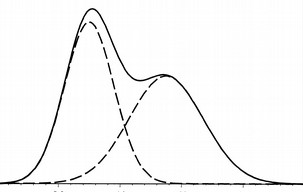
\includegraphics[scale=0.5]{images/mixture.png} }
        \caption{A mixture of two Gaussian distributions, with components shown
        dashed.}
    \end{figure}
    Mixtures of more Gaussian distributions in higher dimensions are defined
    analogously.  Note that because the space of distributions over the real
    line is not finite dimensional, this example does not formally fit under our
    framework; the relevant constructions, however, generalize easily.
    \end{example}

    Mixture models correspond to a relatively well-studied object in algebraic
    geometry.  (For definitions of terms, see Appendix \ref{sec:varieties}.)
    \begin{definition}
    The \emph{secant variety} of the affine variety $V \subset \F^n$ is
    \[
        \Sec(V) = \overline{\cdel[\big]{
        \lambda u + (1 - \lambda) v \vbar
        u,v \in V
        \text{ and }
        \lambda \in \F
        }}
    \]
    where the line indicates the closure of the set under the Zariski topology.  
    \end{definition}
    \begin{proposition}[\citep{DSS08}]
    If $M$ is a semialgebraic set, then the secant variety
    $\Sec\pdel[\big]{\overline{M}}$ is the Zariski closure of the mixture
    $\Mixt(M, M)$.
    \end{proposition}

    For a more thorough exposition on mixture models and secant varieties, we
    refer the reader to Chapter 4 of \citep{DSS08}.


\appendix

\chapter{A Little Algebraic Geometry}

    The field of algebraic geometry grew out of the study of curves and surfaces
    determined by polynomials.  In the mid-twentieth century, the foundations of
    the subject were reformulated by Serre, Grothendieck, and others.  The
    techniques of the field are notoriously both abstract and powerful; the
    following quote by the algebraic geometer David Mumford is perhaps telling
    \citep{Mum99}.
    \begin{quote}
        Algebraic geometry seems to have acquired the reputation of being
        esoteric, exclusive, and very abstract, with adherents who are secretly
        plotting to take over all the rest of mathematics.  In one respect this
        last point is accurate.
    \end{quote}
    More recently, the development of algorithmic techniques, e.g. Gröbner
    bases, has spurred interest in the field of computational algebraic
    geometry.  A standard introduction to algebraic geometry from a
    computational perspective is \citep{CLO97}, which covers algebraic varieties
    and Gröbner bases algorithms while assuming a relatively small amount of
    prerequisite knowledge.  The same authors have a graduate text \citep{CLO05}.

    Here, we introduce some classical algebro-geometric objects.  There are
    many good introductory textbooks for algebraic geometry, including
    \citep{Invitation}, \citep{Sha94}, \citep{Hart}, and \citep{Mum99}.

\section{Affine and Projective Varieties}
    \label{sec:varieties}
    Throughout, let $\F$ be a field.  It is useful to think of $\F$ being either
    $\R$ or $\C$.

    Let $\A^n$ be the affine space of dimension $n$ over $\F$ (that is, the
    vector space $\F^n$ where we view neither the choice of basis nor the choice
    of origin as canonical).  A polynomial $f \in \F[x_1, \ldots, x_n]$ can be
    considered as a function on $\A^n$ by simply evaluating the polynomial on
    any given point.

    \begin{definition}
        An \emph{affine algebraic set} is a subset of the affine space $\A^n$
        of the form
        \[
            V(f_1, \ldots, f_m)
            = \cdel[\big]{x \in \A^n \vbar f_i(x) = 0 \quad\text{for all $i$}}
        \]
        for some finite set of polynomials $f_i \in \F[x_1, \ldots, x_n]$.

        An \emph{affine variety} is an irreducible affine algebraic set, i.e. an
        affine algebraic set that cannot be written as the union of two proper
        affine algebraic subsets.
    \end{definition}
    \noindent Instead of a finite set of polynomials, we can equivalently
    consider a finitely generated ideal.  In fact, $\F[x_1,\ldots,x_n]$ is a
    Noetherian ring, so the condition that the ideal be finitely generated
    condition is redundant.

    Given a subset $X \subset \A^n$, we may consider the ideal of polynomials
    vanishing on the subset
    \[
        I(X) = \cdel[\big]{f \in \F[x_1, \ldots, x_n] \vbar f(x) = 0 \quad\text{for
        all $x \in X$}}.
    \]
    Under certain conditions (e.g. if the field is algebraically closed and the
    ideal is \emph{radical}), the operations $V$ and $I$ are inverses of each other.

    \begin{definition}
        The \emph{projective space} of dimension $n$ (usually denoted $\Proj^n$)
        is the space $\F^{n+1}\setminus \{0\}$ under the equivalence relation $x
        \sim \lambda x$ for $x \in \F^{n+1}$ and $0 \ne \lambda \in \F$.  The
        usual affine coordinate system on $\F^{n+1}$ modulo scaling gives
        \emph{homogeneous coordinates} $[x_0: \cdots: x_n]$ on $\Proj^n$.  If
        $\F = \R$ (resp.  $\C$), the homogeneous coordinates give $\Proj^n$ the
        structure of a real (resp.\ complex) manifold.
    \end{definition}

    It also turns out that projective space behaves particularly nicely for the
    purposes of algebraic geometry, for reasons that we will not describe here.
    Instead of arbitrary polynomials, a different collection of `functions' is
    used on projective space.
    \begin{definition}
        A \emph{homogeneous polynomial} in $n+1$ variables of degree $d$ is a
        polynomial of the form $F(x) = \sum a_I x^I$ where $a_I \in \F$ and the
        multi-index ranges over $I = (i_0, \ldots, i_n)$ such that $i_0 + \cdots
        + i_n = d$.  The monomials are defined to be $x^I = x_0^{i_0}\cdots
        x_n^{i_n}$.  A \emph{homogeneous ideal} is an ideal of $\F[x_0, \ldots,
        x_n]$ generated by homogeneous polynomials.
    \end{definition}
    Notice that if $F$ is homogeneous polynomial of degree $d$, then $F(\lambda
    x) = \lambda^d F(x)$ for $\lambda \in \F$.  The zero set of $F$ in $\Proj^n$
    is then well-defined.  It follows that we can define the projective analogue
    of an affine variety.
    \begin{definition}
        A \emph{projective algebraic set} is a subset of the projective space
        $\Proj^n$ of the form
        \[
            V(f_1, \ldots, f_m)
            = \cdel[\big]{x \in \Proj^n \vbar f_i(x) = 0 \quad\text{for all $i$}}
        \]
        for some finite set of homogeneous polynomials $f_i \in \F[x_0,
        \ldots,x_n]$.  A \emph{projective variety} is an irreducible projective
        algebraic set.
    \end{definition}
    As in the affine case, there is a well-behaved correspondence between the
    homogeneous ideals of $\F[x_0, \ldots, x_n]$ and projective varieties.

    Using these varieties, we may define the \emph{Zariski topology} on $\A^n$
    and $\Proj^n$;  the affine (or projective) varieties are the closed sets of
    the topology.  The Zariski topology is a bit unusual as, unless the field is
    finite, no variety is ever a Hausdorff space.

    For the applications encountered in algebraic statistics, we will need to
    venture into real algebraic geometry, the primary objects of which are
    slightly less well-behaved.
    \begin{definition}
        A \emph{semialgebraic set} is any subset of $\R^n$ of the form
        \[
            V = \cdel[\big]{ x \in \R^n \vbar
                f_i(x) = 0, g_j(x) > 0
            \quad\text{for all $i,j$}}
        \]
        for some finite collection of polynomials $f_i, g_j \in \R[x_1, \ldots,
        x_n]$.
    \end{definition}

    A more in-depth investigation into algebraic geometry reveals the central
    importance of rings of functions on spaces, and the need to consider
    arbitrary commutative rings.  This road leads to the theory of schemes,
    which we will neither need nor pursue here.

\chapter{Machine Learning: Tasks and Tools}
    \label{sec:ML}

    The goal of machine learning is to algorithmically use data in order to
    perform specified tasks better.  The emphasis of the field tends to be
    toward large data sets, efficient algorithms, and `non-parametric' models
    with few assumptions.  Machine learning is studied both by computer
    scientists and statisticians.  The text \citep{EOSL} is an excellent overview
    of machine learning from the latter perspective.

\section{Statistical Classification}

    One common task is the classification problem.  Here, observations are
    points in some large, complicated, or high-dimensional space $X$, and the
    task is to assign a class label to an observation $x \in X$.  Class labels
    come from finite set $C$, and have some meaning.  Classification can also be
    viewed as an attempt to approximate a function $f : X \to C$ given a set of
    observations $\{(x_i, f(x_i)\}_{i=1}^n$ as training data.  For this task to
    be feasible, we cannot consider arbitrary functions; there must be a model.

    \begin{example} 
    The MNIST data set of handwritten digits \citep{MNIST} is commonly seen in the
    machine learning literature.
    \begin{figure}[H]
        \centering
    \scalebox{0.8}{
    
\includegraphics{images/mnist_0.png}\,
    
\includegraphics{images/mnist_1.png}\,
    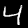
\includegraphics{images/mnist_2.png}\,
    
\includegraphics{images/mnist_3.png}\,
    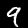
\includegraphics{images/mnist_4.png}
    }
        \caption{Some digits from the MNIST data set.}
    \end{figure}
    \noindent Each $28\times28$ pixel image depicts a handwritten digit $0,
    \ldots, 9$.  The training set contains 60,000 images and the test set
    contains 10,000 images.  An algorithm under evaluation is given the training
    set with correct labels; the task is to correctly label a high percentage of
    the remaining test set.
    \end{example}

    The majority of algorithms in use are in some sense `only a step or two away
    from linear'.  For instance the \emph{perceptron}, a binary linear
    classifier, places observations (which are real vectors) into two classes by
    learning a hyperplane which separates the classes.  The \emph{support vector
    machine} takes a modified approach, as it maps the observed data to a very
    high-dimensional space, and learns a separating hyperplane there.  Another
    common approach is to construct an approximating function as a weighted
    linear combination of a family of basis functions.

    For some problems, however, these techniques may not be sufficient.  Within
    the past ten years, there has been increased interest in so-called `deep
    learning' methods.  An overview of the motivating problems of deep learning
    is contained in \citep{Ben09}.  Perhaps the most influential technique put
    forward so far is the Deep Belief Network.


\section{The Deep Belief Network}
    A Deep Belief Network (DBN) is a generative model consisting essentially a
    stack of RBMs, trained greedily.  The paper \citep{Hin07} introduced a
    technique known as `contrastive divergence' that allowed RBMs, and in turn
    DBNs, to be trained efficiently on problems of practical interest.
    \begin{definition}
    A \emph{Deep Belief Network} is a model on multiple layers of hidden
    variables, built out of RBMs.  Specifically, let $h^k \in \{0,1\}^{n_k}$
    denote the binary state vector of the $k^{\text{th}}$ layer for $0 \le k \le
    m$.  The layer $h^0$ is the visible layer.  The joint distribution of the
    DBN is
    \begin{align*}
        P(v,h^1, \ldots, h^m) &= P(h^{m-1}, h^m) \prod_{k=0}^{m-2} P(h^k \mid h^{k+1})\\
        P(h^k\mid h^{k+1}) &\propto \exp\pdel*{(h^k)^Tb^k + (h^k)^T W^{k+1} h^{k+1}}\\
        P(h^{m-1}, h^{m}) &\propto  \exp\pdel*{(h^{m-1})^T b^k + (h^{m-1})^T W^m
        h^m + (h^m)^T b^m}
    \end{align*}
    for some collection of parameters $b^k$ and $W^k$.
    \end{definition}

    The conditional independence structure of the DBN is described by a graph
    with undirected connections between the top two layers and directed
    connections between all other adjacent layers.
    \begin{figure}[H]
        \centering
        \scalebox{0.6}{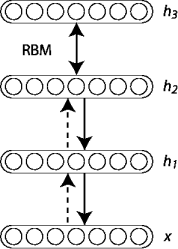
\includegraphics{images/DBN3.png}}
        \caption{Layers of a Deep Belief Network.}
    \end{figure}
    \noindent For classification, the network is greedily trained to represent
    the input data.  The top layer $h^m$ is then trained to classify the inputs
    with a one-hot encoding.  The cited paper reported very low error rates
    (1.25\%) on the MNIST data set using a Deep Belief Network.

% \nocitep{*}

\bibliographystyle{hmcmath}
\bibliography{thesis}

\printindex

\backmatter

\end{document}
